%%%%%%%%%%%%%%%%%%%%%%%%%%%%%%%%%%%%%%%%%%%%%%%%%%%%%%%%%%%%%%%%%%%%%%%%
%% TPI — Analisis de Datos Masivos
%% Etapa 1: Problema, datos y arquitectura
%% Maestria en Ciencias de Datos — UCASAL 2026
%%%%%%%%%%%%%%%%%%%%%%%%%%%%%%%%%%%%%%%%%%%%%%%%%%%%%%%%%%%%%%%%%%%%%%%%

\documentclass[aspectratio=169,11pt]{beamer}

%%%%%%%%%%%%%%%%%%%%%%%%%%%%%%%%%%%%%%%%%%%%%%%%%%%%%%%%%%%%%%%%%%%%%%%%
%% Paquetes
%%%%%%%%%%%%%%%%%%%%%%%%%%%%%%%%%%%%%%%%%%%%%%%%%%%%%%%%%%%%%%%%%%%%%%%%

\usepackage[utf8]{inputenc}
\usepackage[T1]{fontenc}
\usepackage{babel}

\usepackage{amsmath}
\usepackage{amssymb}
\usepackage{booktabs}
\usepackage{tikz}
\usepackage{listings}
\usepackage{xcolor}
\usepackage{pgfpages}
\usepackage{array}
\usepackage{makecell}

\usetikzlibrary{arrows.meta, positioning, shapes.geometric, fit}

%%%%%%%%%%%%%%%%%%%%%%%%%%%%%%%%%%%%%%%%%%%%%%%%%%%%%%%%%%%%%%%%%%%%%%%%
%% Notas del presentador
%% Descomentar la siguiente linea para ver las notas en segunda pantalla
%%%%%%%%%%%%%%%%%%%%%%%%%%%%%%%%%%%%%%%%%%%%%%%%%%%%%%%%%%%%%%%%%%%%%%%%

%\setbeameroption{show notes on second screen=right}

%%%%%%%%%%%%%%%%%%%%%%%%%%%%%%%%%%%%%%%%%%%%%%%%%%%%%%%%%%%%%%%%%%%%%%%%
%% Tema y colores
%%%%%%%%%%%%%%%%%%%%%%%%%%%%%%%%%%%%%%%%%%%%%%%%%%%%%%%%%%%%%%%%%%%%%%%%

\usetheme{Madrid}
\setbeamertemplate{navigation symbols}{}

\definecolor{Azul}{RGB}{30,70,130}
\definecolor{Verde}{RGB}{35,120,80}
\definecolor{Naranja}{RGB}{205,120,20}
\definecolor{Salmon}{RGB}{252,228,214}
\definecolor{AzulClaro}{RGB}{214,228,247}
\definecolor{GrisClaro}{RGB}{242,242,242}

\setbeamercolor{structure}{fg=Azul}

%%%%%%%%%%%%%%%%%%%%%%%%%%%%%%%%%%%%%%%%%%%%%%%%%%%%%%%%%%%%%%%%%%%%%%%%
%% Listings (SQL)
%%%%%%%%%%%%%%%%%%%%%%%%%%%%%%%%%%%%%%%%%%%%%%%%%%%%%%%%%%%%%%%%%%%%%%%%

\lstdefinelanguage{SQL}{
  keywords={SELECT,FROM,JOIN,WHERE,GROUP,BY,HAVING,ORDER,
            LEFT,INNER,WITH,AS,ON,COUNT,AVG,ROUND,FILTER,
            EXPLAIN,ANALYZE,BUFFERS,FORMAT,AND,OR,NOT,IN,
            CAST,EXTRACT,SET},
  keywordstyle=\color{Azul}\bfseries,
  commentstyle=\color{Verde}\itshape,
  stringstyle=\color{Naranja},
  morestring=[b]',
  morecomment=[l]{--},
  sensitive=false
}

\lstset{
  basicstyle=\ttfamily\scriptsize,
  frame=single,
  showstringspaces=false,
  breaklines=true,
  language=SQL
}

%%%%%%%%%%%%%%%%%%%%%%%%%%%%%%%%%%%%%%%%%%%%%%%%%%%%%%%%%%%%%%%%%%%%%%%%

\title{Analisis de Datos Masivos}

\subtitle{
Trabajo Practico Integrador\\
Etapa 1 --- Problema, datos y arquitectura
}

\author{Lic.\ Pablo Daniel Origlia}

\date{Maestria en Ciencias de Datos --- UCASAL 2026}

%%%%%%%%%%%%%%%%%%%%%%%%%%%%%%%%%%%%%%%%%%%%%%%%%%%%%%%%%%%%%%%%%%%%%%%%

\begin{document}

%%%%%%%%%%%%%%%%%%%%%%%%%%%%%%%%%%%%%%%%%%%%%%%%%%%%%%%%%%%%%%%%%%%%%%%%
%% SLIDE 1: PORTADA
%%%%%%%%%%%%%%%%%%%%%%%%%%%%%%%%%%%%%%%%%%%%%%%%%%%%%%%%%%%%%%%%%%%%%%%%

\begin{frame}

\titlepage

\note{
Presentacion de avance de la Etapa 1 del TPI. Duracion: 5-7 minutos.
Estructura: problema que abordamos (1 slide), arquitectura de datos
(1 slide), hallazgos del import (1 slide), las 5 preguntas analiticas
(1 slide), resultados de performance (2 slides) y cierre con lo que
viene (1 slide). Total: 8 slides sin contar portada.
}

\end{frame}

%%%%%%%%%%%%%%%%%%%%%%%%%%%%%%%%%%%%%%%%%%%%%%%%%%%%%%%%%%%%%%%%%%%%%%%%
%% SLIDE 2: PROBLEMA Y PREGUNTA CENTRAL
%%%%%%%%%%%%%%%%%%%%%%%%%%%%%%%%%%%%%%%%%%%%%%%%%%%%%%%%%%%%%%%%%%%%%%%%

\begin{frame}

\frametitle{El problema que abordamos}

\begin{block}{Pregunta central}
\textbf{i,Como impactan las condiciones operativas de la flota}
(tipo de vehiculo, conductor, incidentes, mantenimiento)
\textbf{sobre los tiempos de entrega y la satisfaccion del cliente}
en un operador de e-commerce brasileno?
\end{block}

\vspace{4mm}

\begin{columns}[T]

\column{0.48\textwidth}
\textbf{Por que este problema}
\begin{itemize}
\item Olist expone el \textit{resultado} logistico (demoras, resenas)
pero no las \textit{causas} operativas
\item Cruzar ambas fuentes permite pasar de descripcion a causas
\item Decisiones concretas: mantenimiento preventivo, asignacion
de rutas, gestion de conductores
\end{itemize}

\column{0.48\textwidth}
\textbf{Tipo de analisis previsto}
\begin{itemize}
\item \textbf{Descriptivo}: patrones de demora por region y vehiculo
\item \textbf{Predictivo}: modelo de riesgo de entrega tarde
(Etapas 3 y 4)
\item \textbf{Prescriptivo}: recomendaciones de asignacion
(Etapa 4)
\end{itemize}

\end{columns}

\note{
El punto clave a comunicar: Olist solo nos dice "esta orden llego
tarde y el cliente puso 2 estrellas". No nos dice POR QUE llego
tarde. La flota sintetica que construimos nos da la capa de causas:
tipo de vehiculo, comportamiento del conductor, nivel de riesgo de
la ruta. La combinacion de las dos fuentes es lo que hace interesante
el proyecto. Mencionar brevemente que el dataset de flota es sintetico
pero calibrado con distribuciones reales de un dataset de Kaggle
(dynamic supply chain logistics).
}

\end{frame}

%%%%%%%%%%%%%%%%%%%%%%%%%%%%%%%%%%%%%%%%%%%%%%%%%%%%%%%%%%%%%%%%%%%%%%%%
%% SLIDE 3: ARQUITECTURA DE DATOS
%%%%%%%%%%%%%%%%%%%%%%%%%%%%%%%%%%%%%%%%%%%%%%%%%%%%%%%%%%%%%%%%%%%%%%%%

\begin{frame}

\frametitle{Arquitectura de datos}

\begin{columns}[T]

\column{0.52\textwidth}

\textbf{Fuente 1 --- Olist} \hfill {\small (real, Kaggle)}

\vspace{1mm}

\begin{tabular}{@{}lrr@{}}
\toprule
Tabla & Filas \\
\midrule
olist\_geolocation & 1.000.163 \\
olist\_orders & 99.441 \\
olist\_order\_items & 112.650 \\
olist\_order\_reviews & 99.224 \\
olist\_order\_payments & 103.886 \\
olist\_customers + sellers & 102.536 \\
olist\_products & 32.952 \\
\bottomrule
\end{tabular}

\vspace{3mm}

\column{0.44\textwidth}

\textbf{Fuente 2 --- Flota} \hfill {\small (sintetica calibrada)}

\vspace{1mm}

\begin{tabular}{@{}lr@{}}
\toprule
Tabla & Filas \\
\midrule
fleet\_deliveries & 96.470 \\
fleet\_incidents & 3.574 \\
fleet\_maintenance & 688 \\
fleet\_vehicles & 60 \\
fleet\_drivers & 40 \\
\bottomrule
\end{tabular}

\vspace{3mm}

\begin{block}{\small Clave de vinculacion}
\texttt{\small fleet\_deliveries.order\_id}\\
\texttt{\small = olist\_orders.order\_id}
\end{block}

\end{columns}

\vspace{2mm}

{\small
\textbf{SGBD:} PostgreSQL 15 \quad
\textbf{Total:} $\approx$1,6 M registros \quad
\textbf{Indices:} 67 (DDL + covering indexes)
}

\note{
Los datos estan en una base PostgreSQL local. La tabla central de
vinculacion es fleet_deliveries: tiene una fila por cada orden
de Olist con status='delivered', con el vehiculo y conductor asignado,
la distancia estimada, y las dos variables objetivo de los modelos
predictivos (eta_variation_hours y delivery_status on_time/delayed).
El script generate_fleet_dataset.py calibra sus distribuciones
con el dataset de Kaggle de telemetria logistica. El total de ~1.6M
registros justifica el enfoque de "datos masivos": en especial
olist_geolocation con 1M de filas es el principal driver de I/O
en las consultas.
}

\end{frame}

%%%%%%%%%%%%%%%%%%%%%%%%%%%%%%%%%%%%%%%%%%%%%%%%%%%%%%%%%%%%%%%%%%%%%%%%
%% SLIDE 4: HALLAZGOS DEL IMPORT (calidad de datos)
%%%%%%%%%%%%%%%%%%%%%%%%%%%%%%%%%%%%%%%%%%%%%%%%%%%%%%%%%%%%%%%%%%%%%%%%

\begin{frame}

\frametitle{Calidad de datos --- hallazgos del import}

El dataset Olist presento \textbf{4 problemas conocidos} que
requirieron fixes antes del import (\texttt{03b\_fix\_constraints.sql}):

\vspace{3mm}

\begin{tabular}{@{}p{3.6cm}p{4.4cm}p{4.0cm}@{}}
\toprule
Problema & Causa & Solucion aplicada \\
\midrule
Coordenadas fuera de Brasil &
42 de 1M registros en geolocation &
CHECK eliminado; filtrar en Etapa 2 \\

\addlinespace

Productos con peso = 0 &
4 registros con weight\_g = 0 &
CHECK ampliado; imputar mediana \\

\addlinespace

Items con producto inexistente &
Productos eliminados del catalogo &
Placeholder \texttt{unknown\_product} \\

\addlinespace

review\_id duplicados &
814 duplicados en CSV (bug Olist) &
Nueva PK interna \texttt{review\_pk} \\
\bottomrule
\end{tabular}

\vspace{4mm}

\begin{columns}[T]
\column{0.48\textwidth}
{\small \color{Verde}$\checkmark$} \textbf{8 ordenes} con
\texttt{status='delivered'} pero sin fecha real de entrega
(excluir en Etapa 2)

\column{0.48\textwidth}
{\small \color{Verde}$\checkmark$} Todos los problemas
\textbf{documentados} en \texttt{03c\_post\_import.sql}
y en el diccionario de datos (v2)
\end{columns}

\note{
Este slide es importante para la evaluacion: muestra que el grupo
hizo un diagnostico de calidad de datos real, no solo cargamos
los CSV y listo. Los 4 problemas son bugs conocidos del dataset
Olist, no errores nuestros. Lo relevante academicamente es que
los identificamos, documentamos la decision de fix y dejamos
registro para Etapa 2. Destacar que el 03c_post_import.sql es
el insumo directo del notebook de limpieza de Etapa 2.
}

\end{frame}

%%%%%%%%%%%%%%%%%%%%%%%%%%%%%%%%%%%%%%%%%%%%%%%%%%%%%%%%%%%%%%%%%%%%%%%%
%% SLIDE 5: PREGUNTAS ANALITICAS
%%%%%%%%%%%%%%%%%%%%%%%%%%%%%%%%%%%%%%%%%%%%%%%%%%%%%%%%%%%%%%%%%%%%%%%%

\begin{frame}

\frametitle{Las 5 preguntas analiticas}

\begin{enumerate}

\item \textbf{Q1} --- i,Que factores operativos
(\texttt{route\_risk\_level}, tipo de vehiculo,
\texttt{driver\_behavior\_score}) se asocian a las entregas
demoradas, por estado de Brasil?

\vspace{2mm}

\item \textbf{Q2} --- i,Existe relacion entre el comportamiento
del conductor y el score promedio de resena del cliente?

\vspace{2mm}

\item \textbf{Q3} --- i,En que meses se concentran los
mantenimientos correctivos, y coincide con el pico de
ordenes demoradas en Olist?

\vspace{2mm}

\item \textbf{Q4} --- i,Que tipos de incidente generan mayor
impacto en horas de demora?

\vspace{2mm}

\item \textbf{Q5} --- i,El costo de mantenimiento por tipo
de vehiculo se justifica con su rendimiento logistico?

\end{enumerate}

\note{
Mencionar brevemente que estas 5 preguntas guian tanto las consultas
SQL de Etapa 1 como los modelos predictivos de Etapa 3. Q2 anticipa
el Modelo 2 (clasificacion de delivery_status). Q3 valida la
hipotesis de estacionalidad que construimos en el script de
generacion: el patron nov-dic de mantenimientos correctivos deberia
aparecer en los datos. Q5 es la unica consulta 100% interna a las
tablas de flota, lo que permite compararla con Q1 (que cruza Olist)
para demostrar el costo de los JOINs entre fuentes.
}

\end{frame}

%%%%%%%%%%%%%%%%%%%%%%%%%%%%%%%%%%%%%%%%%%%%%%%%%%%%%%%%%%%%%%%%%%%%%%%%
%% SLIDE 6: ANALISIS DE PERFORMANCE (tabla)
%%%%%%%%%%%%%%%%%%%%%%%%%%%%%%%%%%%%%%%%%%%%%%%%%%%%%%%%%%%%%%%%%%%%%%%%

\begin{frame}

\frametitle{Analisis de performance --- EXPLAIN ANALYZE}

\begin{center}

\footnotesize

\begin{tabular}{@{}lrrrrll@{}}
\toprule
Consulta &
\makecell{Exec.\\ sin (ms)} &
\makecell{Exec.\\ con (ms)} &
Mejora &
\makecell{Sh. read\\ sin} &
Operacion principal &
Indice usado \\
\midrule
Q1 Estado $\times$ vehiculo &
184 & 164 & \textcolor{Verde}{$-$10.9\%} &
1.496 & Sort + Parallel Hash Join & ninguno \\

Q2 Conductor $\leftrightarrow$ resena &
145 & 107 & \textcolor{Verde}{$-$26.5\%} &
0 & Sort + Parallel Hash Join & ninguno \\

Q3 Estacionalidad &
218 & 173 & \textcolor{Verde}{$-$20.4\%} &
0 & Sort + Hash Join & ninguno* \\

Q4 Incidentes &
43 & 36 & \textcolor{Verde}{$-$17.0\%} &
2 & Sort + Nested Loop & \texttt{idx\_del\_status} \\

Q5 Costo vs.\ rendimiento &
57 & 62 & \textcolor{Naranja}{$+$8.3\%} &
0 & Merge Join & ninguno \\
\bottomrule
\end{tabular}

\end{center}

\vspace{1mm}
{\footnotesize * Q3 hace \textbf{spill a disco} (718 bloques temp):
\texttt{SET work\_mem = '16MB'} lo elimina.}

\vspace{2mm}

{\footnotesize \textbf{Tamano de indices vs.\ datos:}
\texttt{olist\_orders} 59\,MB datos / 45\,MB indices (76\,\%) \quad
\texttt{fleet\_deliveries} 68\,MB datos / 55\,MB indices (81\,\%)}

\note{
Este slide es el corazon del analisis de performance de Etapa 1.
Puntos clave a comunicar: (1) el planner rechazo casi todos los
covering indexes nuevos porque las consultas necesitan el 40-97%
de las filas: a ese volumen un Seq Scan paralelo gana. Esto es
comportamiento correcto del optimizador, no un fallo de diseno.
(2) La mejora en Q2 (26.5%) se debe principalmente al calentamiento
de cache entre ejecuciones, no a los indices. (3) Q5 es la mas
interesante conceptualmente: empeora con indices porque el overhead
de planning supera el beneficio. Demuestra que mas indices no siempre
es mejor. (4) El ratio indice/datos de ~80% es alto: el
idx_del_analytical_base de 11MB es candidato a eliminar.
}

\end{frame}

%%%%%%%%%%%%%%%%%%%%%%%%%%%%%%%%%%%%%%%%%%%%%%%%%%%%%%%%%%%%%%%%%%%%%%%%
%% SLIDE 7: HALLAZGOS DE PERFORMANCE (conclusiones)
%%%%%%%%%%%%%%%%%%%%%%%%%%%%%%%%%%%%%%%%%%%%%%%%%%%%%%%%%%%%%%%%%%%%%%%%

\begin{frame}

\frametitle{Que nos dice el planner}

\begin{columns}[T]

\column{0.48\textwidth}

\textbf{Lo que observamos}

\begin{itemize}

\item El planner uso Seq Scan en 4 de 5 consultas aunque
los covering indexes existian

\item Unico indice activo: \texttt{idx\_del\_status}
(Bitmap Scan, 624\,kB, Q4)

\item Q3 hace spill a disco por \texttt{work\_mem}
insuficiente (4\,MB default)

\item Q5 \textbf{empeora} 8\,\% con mas indices
(overhead de planning)

\end{itemize}

\column{0.48\textwidth}

\textbf{Por que importa}

\begin{itemize}

\item Cuando un filtro devuelve $>$10--15\,\% de las filas,
el Seq Scan paralelo gana al Index Scan

\item Mas indices $\neq$ mejor performance

\item Los covering indexes de Secciones A--E entraran en
accion en Etapa 2 (dataset analitico, mayor selectividad)

\item El indice con mejor relacion tamano/impacto
del proyecto: \texttt{idx\_del\_status} (Bitmap Scan)

\end{itemize}

\end{columns}

\vspace{3mm}

\begin{block}{Aprendizaje central}
El optimizador de PostgreSQL elige correctamente entre Seq Scan e
Index Scan segun el volumen de filas a recuperar. Disenamos
bien los indices; el dataset todavia no tiene la selectividad
suficiente para que todos sean necesarios.
\end{block}

\note{
Este slide responde la pregunta implicita del evaluador: "si los
indices no se usaron, i,para que los crearon?". La respuesta es
que (a) para las consultas analiticas de Etapa 1 el planner tomo
la decision correcta, (b) los covering indexes de Secciones A-E
se van a activar en Etapa 2 cuando el dataset analitico tenga
filtros mas selectivos (ej: por region especifica o por tipo de
vehiculo), y (c) el ejercicio de medir antes y despues es lo que
pide el enunciado, independientemente del resultado. La regresion
en Q5 es el hallazgo mas rico academicamente: ilustra el trade-off
espacio/velocidad del enunciado de forma concreta.
}

\end{frame}

%%%%%%%%%%%%%%%%%%%%%%%%%%%%%%%%%%%%%%%%%%%%%%%%%%%%%%%%%%%%%%%%%%%%%%%%
%% SLIDE 8: ESTADO DE ENTREGABLES
%%%%%%%%%%%%%%%%%%%%%%%%%%%%%%%%%%%%%%%%%%%%%%%%%%%%%%%%%%%%%%%%%%%%%%%%

\begin{frame}

\frametitle{Entregables de Etapa 1}

\begin{columns}[T]

\column{0.48\textwidth}

\textbf{Completados} {\small \color{Verde}$\checkmark$}

\begin{itemize}
\item Base de datos cargada (PostgreSQL 15)
\item DDL con constraints, FKs y 67 indices
\item Fix de 4 problemas de calidad del dataset
\item Script de generacion de flota sintetica
(\texttt{generate\_fleet\_dataset.py} v1.1)
\item 5 consultas analiticas con EXPLAIN ANALYZE
(sin y con indices)
\item Analisis de performance documentado
\item Diccionario de datos v2 (14 tablas, 14 KPIs,
relaciones)
\end{itemize}

\column{0.48\textwidth}

\textbf{Anticipaciones para Etapa 2}

\begin{itemize}
\item Diagnostico de calidad listo (\texttt{03c}):\\
coordenadas invalidas, pesos nulos,\\
duplicados en reviews, 8 ordenes sin fecha
\item Indices F1 y F2 creados anticipadamente\\
para el JOIN principal del dataset analitico
\item Variables objetivo ya definidas:\\
\texttt{eta\_variation\_hours} (regresion)\\
\texttt{delivery\_status} (clasificacion)
\end{itemize}

\vspace{3mm}

\begin{block}{\small Repositorio}
{\footnotesize \texttt{github.com/pablo-origlia/}\\
\texttt{tpi-logistica-ecommerce}}
\end{block}

\end{columns}

\note{
Este slide sirve para mostrar que el grupo no solo hizo lo minimo
que pide el enunciado sino que anticipo trabajo de Etapa 2. El
diagnostico de calidad en 03c es directamente el insumo del notebook
01_limpieza.ipynb. Los indices F1 y F2 se crearon pensando en la
consulta de generacion del dataset analitico, no en las consultas
de Etapa 1. Las variables objetivo ya estan definidas y documentadas
en el diccionario, lo que simplifica la Etapa 3.
}

\end{frame}

%%%%%%%%%%%%%%%%%%%%%%%%%%%%%%%%%%%%%%%%%%%%%%%%%%%%%%%%%%%%%%%%%%%%%%%%
%% SLIDE 9: CIERRE Y PROXIMOS PASOS
%%%%%%%%%%%%%%%%%%%%%%%%%%%%%%%%%%%%%%%%%%%%%%%%%%%%%%%%%%%%%%%%%%%%%%%%

\begin{frame}

\frametitle{Proximos pasos --- Etapa 2}

\begin{columns}[T]

\column{0.52\textwidth}

\textbf{Dataset analitico}

\begin{enumerate}

\item Imputar pesos nulos (mediana por categoria)
\item Filtrar coordenadas fuera de Brasil
\item Excluir 8 ordenes sin \texttt{delivery\_date}
\item Construir el JOIN principal:\\
14 tablas $\rightarrow$ 1 dataset analitico

\end{enumerate}

\vspace{3mm}

\textbf{Analisis exploratorio (EDA)}

\begin{itemize}
\item Distribucion de \texttt{eta\_variation\_hours}
\item Correlacion conductor $\leftrightarrow$ resena
\item Estacionalidad de mantenimientos nov--dic
\item Segmentacion por tipo de vehiculo y region
\end{itemize}

\column{0.44\textwidth}

\vspace{2mm}

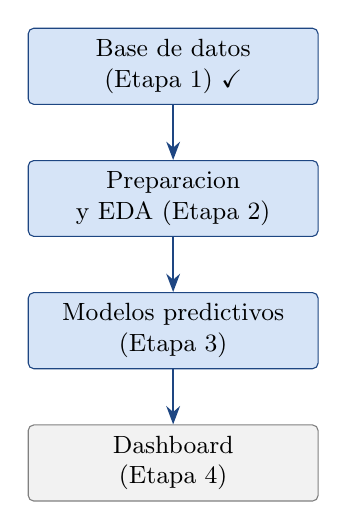
\begin{tikzpicture}[
  node distance=7mm,
  box/.style={
    draw=Azul, rounded corners=2pt,
    fill=AzulClaro, text width=3.4cm,
    align=center, font=\small,
    inner sep=4pt
  },
  arr/.style={->, >=Stealth, Azul, thick}
]

\node[box] (bbdd) {Base de datos\\ (Etapa 1) \checkmark};
\node[box, below=of bbdd] (prep)
  {Preparacion\\ y EDA (Etapa 2)};
\node[box, below=of prep] (modelos)
  {Modelos predictivos\\ (Etapa 3)};
\node[box, below=of modelos, fill=GrisClaro, draw=gray]
  (dash) {Dashboard\\ (Etapa 4)};

\draw[arr] (bbdd) -- (prep);
\draw[arr] (prep) -- (modelos);
\draw[arr] (modelos) -- (dash);

\end{tikzpicture}

\end{columns}

\note{
Slide de cierre. El objetivo es mostrar que la Etapa 1 no es un
fin en si mismo sino la base de todo lo que viene. El diagrama
TikZ muestra el pipeline completo: ya terminamos el primer bloque
(verde) y el proximo es Etapa 2. Frase de cierre sugerida: "La
Etapa 1 nos dio la base de datos limpia, documentada y con los
problemas de calidad identificados. En la Etapa 2 vamos a
construir el dataset analitico que alimenta los modelos. Las
variables objetivo ya estan definidas: eta_variation_hours para
regresion y delivery_status para clasificacion."
}

\end{frame}

%%%%%%%%%%%%%%%%%%%%%%%%%%%%%%%%%%%%%%%%%%%%%%%%%%%%%%%%%%%%%%%%%%%%%%%%

\end{document}
